\section{Grammaires et analyse syntaxique}
The lexeur turns a stream of characters into a stream of lexèmes; the
\textit{parseur} turns that stream of lexèmes into a tree. This chapter is about
the second step, and about the objects that make it possible: grammaires
formelles, the restriction to grammaires non contextuelles that makes the
problème de l'appartenance decidable at all, ambiguity and how a grammar is
rewritten to remove it, a cubic-time recognition algorithm together with a full
hand-run trace of it, and finally the linear-time restriction --- LL(1) --- that
real compilateurs actually use. The chapter is written top-down in the sense
that it starts with the most general
object and removes power at every step, because every restriction buys
something: decidability, then polynomial time, then linear time.

\subsection{Grammaires formelles}

\begin{definition}[Grammaire formelle]
  Une \textbf{grammaire formelle} (\textit{formal grammar}) c'est :
  \begin{itemize}
    \item un ensemble de \textbf{symboles terminaux} (\textit{terminal
      symbols}) souvent noté $\Sigma$ ;
    \item un ensemble de \textbf{symboles non-terminaux} (\textit{non-terminal
      symbols}), noté $N$ ;
    \item un \textbf{symbole de départ} (\textit{start symbol}) $S$ ;
    \item un ensemble de \textbf{règles de production} (\textit{production
      rules}) $(\Sigma \union N)^{+} \to (\Sigma \union N)^{*}$.
  \end{itemize}
\end{definition}

\begin{notation}
  On donne souvent les symboles $\Sigma$ en minuscules et ceux de $N$ en
  majuscules. La grammaire est donc \emph{juste un ensemble de règles} ---
  $\Sigma$, $N$ and $S$ are read off the rules themselves.
\end{notation}

The left-hand side of a rule is a non-empty \emph{mot} of symbols, not a
single non-terminal. That is the whole generality of the definition, and it is
exactly what will be given up in the next subsection.

\begin{example}[A grammar that is not context-free]
  $S \to aSb$, \quad $S \to \epsilon$, \quad $ab \to ba$.
\end{example}

\begin{definition}[Langage d'une grammaire]
  Le \textbf{langage} $L(G)$ d'une grammaire $G$ c'est l'ensemble des mots de
  $\Sigma^{*}$ que l'on peut obtenir en appliquant des \textbf{règles de
  réécriture} (\textit{rewriting rules}) depuis la chaîne contenant $S$ (and
  nothing else).
\end{definition}

\begin{example}[$aababb$ belongs to the language above]
  $aababb$ est dans le langage de $S \to aSb$, $ab \to ba$ car
  \[
    S \to aSb \to aaSbb \to aaaSbbb \to aaabbb \to aababb .
  \]
  The first three steps use $S \to aSb$, the fourth uses $S \to \epsilon$, and
  the last one uses $ab \to ba$ on the middle of $aaabbb$.
\end{example}

\begin{remark}
  Quel est le langage des mots reconnus par cette grammaire ? The answer is the
  set of words over $\{a,b\}$ containing as many $a$ as
  $b$: the first two rules generate exactly $a^{n}b^{n}$, and $ab \to ba$ lets a
  $b$ migrate leftwards past an $a$ as often as one likes, which reaches every
  arrangement of $n$ letters $a$ and $n$ letters $b$ (run the rule backwards and
  one is merely bubble-sorting the word into $a^{n}b^{n}$). The rule
  $ab \to ba$ can never fire before the $S$ is gone, since no mot containing
  $S$ has an $a$ immediately followed by a $b$.
\end{remark}

\subsubsection{Le problème de l'appartenance}
\begin{problem}[Problème de l'appartenance (\textit{membership problem})]
  Étant donné $w$ et $G$, décider si $w \in L(G)$.
\end{problem}

\begin{theorem}
  For general grammaires formelles the problème de l'appartenance is
  \textbf{indécidable} (\textit{undecidable}).
\end{theorem}

\noindent $\Rightarrow$ on va devoir restreindre l'ensemble des grammaires. Il
existe plusieurs restrictions utiles et étudiées. The rest of the chapter is a
tour of the two that matter for a compilateur.

\subsection{Grammaires non contextuelles}

\begin{definition}[Grammaire non contextuelle]
  Une \textbf{grammaire non contextuelle} (\textit{context-free grammar}, CFG)
  ou \textit{grammaire hors-contexte} ou \textit{grammaire algébrique} c'est une
  grammaire dans laquelle les règles de production sont toutes de la forme
  \[
    N \to (\Sigma \union N)^{*} .
  \]
\end{definition}

The name says what has been given up: the left-hand side is a single
non-terminal, so a rule may be applied to an occurrence of $N$ \emph{without
looking at its context}. The grammar $ab \to ba$ of the previous subsection is
excluded.

\begin{example}
  $S \to S + S$, \quad $S \to S * S$, \quad $S \to 1$.
\end{example}

\noindent For this class the problème de l'appartenance is
\textbf{décidable et polynomial} --- the algorithm and its exponent are the
subject of the next two subsections.

\subsubsection{Arbre de dérivation}
\begin{definition}[Arbre de dérivation]
  Pour $G$ une CFG, un \textbf{arbre de dérivation} (\textit{derivation tree}),
  c'est un arbre $A$ dans lequel :
  \begin{itemize}
    \item les feuilles sont étiquetées par des terminaux ;
    \item les nœuds internes sont étiquetés par des non-terminaux ;
    \item la racine est étiquetée par $S$ ;
    \item les enfants $n_{1} \dots n_{k}$ d'un nœud étiqueté par $X$ doivent
      être étiquetés par $s_{1} \dots s_{k}$ tel que
      $X \to s_{1} \dots s_{k} \in G$.
  \end{itemize}
  Le \textbf{mot de $A$} c'est le mot des étiquettes des feuilles dans l'ordre.
\end{definition}

\begin{remark}
  $w \in L(G)$ si et seulement si $w$ est le mot d'un arbre de dérivation. On
  dit qu'une grammaire est \textbf{non-ambiguë} (\textit{unambiguous}) s'il
  existe un \emph{unique} arbre de dérivation pour chaque mot.
\end{remark}

The arbre de dérivation, not the derivation, is the object a compilateur wants:
the order in which the rules were applied is irrelevant, the shape of the tree
is the meaning. A word with two arbres de dérivation is a program with two
meanings.

\begin{figure}[h!]
  \centering
  \begin{tikzpicture}[font=\small, level distance=0pt]
    % ---- left tree : 0*1+1 grouped as 0*(1+1)
    \begin{scope}[xshift=0cm]
      \node (a)  at (2.0, 3.0) {$S$};
      \node (b)  at (0.6, 2.1) {$S$};
      \node (c)  at (2.0, 2.1) {$*$};
      \node (d)  at (3.4, 2.1) {$S$};
      \node (e)  at (0.6, 1.2) {$0$};
      \node (f)  at (3.4, 1.2) {$S$};
      \node (g)  at (2.4, 0.3) {$S$};
      \node (h)  at (3.4, 0.3) {$+$};
      \node (i)  at (4.4, 0.3) {$S$};
      \node (j)  at (2.4,-0.6) {$1$};
      \node (k)  at (4.4,-0.6) {$1$};
      \foreach \u/\v in {a/b,a/c,a/d,b/e,d/f,f/g,f/h,f/i,g/j,i/k}
        { \draw (\u) -- (\v); }
      \node[font=\footnotesize] at (2.2,-1.3) {$0*(1+1)$};
    \end{scope}
    % ---- right tree : 0*1+1 grouped as (0*1)+1
    \begin{scope}[xshift=7.4cm]
      \node (A)  at (2.4, 3.0) {$S$};
      \node (B)  at (1.2, 2.1) {$S$};
      \node (C)  at (2.4, 2.1) {$+$};
      \node (D)  at (3.6, 2.1) {$S$};
      \node (E)  at (1.2, 1.2) {$S$};
      \node (F)  at (3.6, 1.2) {$1$};
      \node (G)  at (0.2, 0.3) {$S$};
      \node (H)  at (1.2, 0.3) {$*$};
      \node (I)  at (2.2, 0.3) {$S$};
      \node (J)  at (0.2,-0.6) {$0$};
      \node (K)  at (2.2,-0.6) {$1$};
      \foreach \u/\v in {A/B,A/C,A/D,B/E,D/F,E/G,E/H,E/I,G/J,I/K}
        { \draw (\u) -- (\v); }
      \node[font=\footnotesize] at (2.0,-1.3) {$(0*1)+1$};
    \end{scope}
  \end{tikzpicture}
\end{figure}

\noindent Both trees have word $0*1+1$, so the grammar
$S \to S+S \mid S*S \mid 1 \mid 0$ is ambiguous, and it is ambiguous in the
worst possible way: the two trees are the two different arithmetic values.

\begin{remark}
  The same grammar has smaller trees, and their words are read off the leaves
  in the same way. The tree $S \to S + S$ whose left child derives $1$ and whose
  right child derives $0$ has a $0$ as its right leaf, so its word is $1+0$.
  The two trees above both have word $0*1+1$, as their leaves show.
\end{remark}

\subsection{Grammaire ambiguë}

On s'attend en général à ce que la structure des programmes écrits ne soit pas
ambiguë. The canonical counter-example is the dangling \verb|else|:

\begin{lstlisting}[language=C]
if(cond1)
  if (cond2)
    printf("a");
else
    print("b");
\end{lstlisting}

\begin{center}
  \begin{tabular}{c c c}
    \toprule
    \verb|cond1| & \verb|cond2| & affichage \\
    \midrule
    Vrai  & Vrai  & ``a'' \\
    Vrai  & Faux  & ? \\
    Faux  & \dots & ? \\
    \bottomrule
  \end{tabular}
\end{center}

\noindent The indentation suggests the \verb|else| belongs to the outer
\verb|if|; the language says otherwise. \textbf{La syntaxe du C est claire, le
\texttt{else} se raccroche au \texttt{if} le plus imbriqué.} The code therefore
parses as\newline \verb|if(cond1) { if(cond2) printf("a"); else print("b"); }|, so the
second row prints \verb|"b"| --- the inner \verb|else| fires --- and the third row
prints nothing at all, the whole outer statement being skipped. These are the
answers the rule forces in the two \verb|?| cells of the table. That the rule
has to be stated at all is a decision
the language designer had to take, and it has to be forced by the grammar rather
than by a footnote.

\subsubsection{Modéliser le \texttt{else} ambigu}
Modélisons l'exemple \verb|if if printf else printf|. Grammaire :
\[
  S \to \texttt{printf}, \qquad
  S \to \texttt{if}\, S, \qquad
  S \to \texttt{if}\, S\ \texttt{else}\, S .
\]

\begin{figure}[h!]
  \centering
  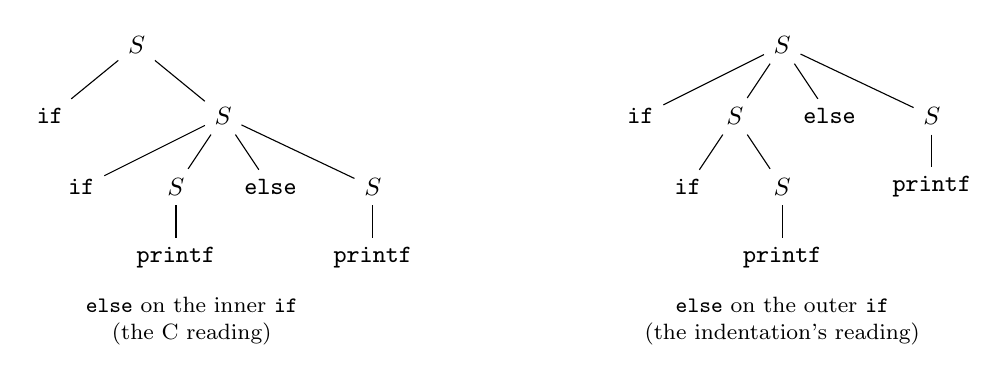
\begin{tikzpicture}[font=\small]
    % ---- else attaches to the inner if
    \begin{scope}
      \node (a) at (1.6, 2.7) {$S$};
      \node (b) at (0.5, 1.8) {\texttt{if}};
      \node (c) at (2.7, 1.8) {$S$};
      \node (d) at (0.9, 0.9) {\texttt{if}};
      \node (e) at (2.1, 0.9) {$S$};
      \node (f) at (3.3, 0.9) {\texttt{else}};
      \node (g) at (4.6, 0.9) {$S$};
      \node (h) at (2.1, 0.0) {\texttt{printf}};
      \node (i) at (4.6, 0.0) {\texttt{printf}};
      \foreach \u/\v in {a/b,a/c,c/d,c/e,c/f,c/g,e/h,g/i} { \draw (\u) -- (\v); }
      \node[font=\footnotesize, align=center] at (2.3,-0.8)
        {\texttt{else} on the inner \texttt{if}\\ (the C reading)};
    \end{scope}
    % ---- else attaches to the outer if
    \begin{scope}[xshift=7.6cm]
      \node (A) at (2.2, 2.7) {$S$};
      \node (B) at (0.4, 1.8) {\texttt{if}};
      \node (C) at (1.6, 1.8) {$S$};
      \node (D) at (2.8, 1.8) {\texttt{else}};
      \node (E) at (4.1, 1.8) {$S$};
      \node (F) at (1.0, 0.9) {\texttt{if}};
      \node (G) at (2.2, 0.9) {$S$};
      \node (H) at (4.1, 0.9) {\texttt{printf}};
      \node (I) at (2.2, 0.0) {\texttt{printf}};
      \foreach \u/\v in {A/B,A/C,A/D,A/E,C/F,C/G,E/H,G/I} { \draw (\u) -- (\v); }
      \node[font=\footnotesize, align=center] at (2.2,-0.8)
        {\texttt{else} on the outer \texttt{if}\\ (the indentation's reading)};
    \end{scope}
  \end{tikzpicture}
\end{figure}

\begin{problem}[Exercice --- rendre la grammaire non ambiguë]
  Modifier la grammaire pour la rendre non ambiguë.
\end{problem}

\begin{example}[Solution]
  \[
    \begin{aligned}
      S  &\to \texttt{if}\, S       & \qquad IE &\to \texttt{printf} \\
      S  &\to IE                    & \qquad IE &\to \texttt{if}\, IE\ \texttt{else}\, S
    \end{aligned}
  \]
  A new non-terminal $IE$ is introduced and the then-branch of an
  \verb|if|\dots\verb|else| is restricted to it: only $IE$, never $S$, may sit
  between an \verb|if| and its \verb|else|. That is what puts the \verb|else| on
  the inner \verb|if| in the tree below, and it disambiguates the example the
  exercise was set on.
\end{example}

\begin{remark}
  It does \emph{not} disambiguate the grammar in general, and it is worth seeing
  why, because the tempting justification --- that $IE$ is \emph{closed}, i.e.\
  cannot swallow a following \verb|else| --- is false. The rule
  $IE \to \texttt{if}\, IE\ \texttt{else}\, S$ ends in $S$, and $S \to
  \texttt{if}\, S$, so an $IE$ can itself end in an unmatched \verb|if|. The
  shortest witness is
  \[ \texttt{if if printf else if printf else printf} \]
  which still has \textbf{two} arbres de dérivation: the final \verb|else| can
  bind the third \verb|if| (via $S \to \texttt{if}\, S$ with the inner $S$ an $IE$),
  or bind the outermost one (via $S \to IE$ with
  $\texttt{if if printf else if printf}$ derived as the inner $IE$), leaving the
  third \verb|if| dangling. Every shorter mot has a unique tree, which is why
  a single illustrative derivation, like the one drawn below, looks conclusive.
  Closing the construction properly requires the else-branch to be closed too:
  $IE \to \texttt{if}\, IE\ \texttt{else}\, IE$.
\end{remark}

\begin{figure}[h!]
  \centering
  \begin{tikzpicture}[font=\small]
    \node (a) at (1.8, 3.6) {$S$};
    \node (b) at (0.6, 2.7) {\texttt{if}};
    \node (c) at (3.0, 2.7) {$S$};
    \node (d) at (3.0, 1.8) {$IE$};
    \node (e) at (1.1, 0.9) {\texttt{if}};
    \node (f) at (2.4, 0.9) {$IE$};
    \node (g) at (3.6, 0.9) {\texttt{else}};
    \node (h) at (5.0, 0.9) {$S$};
    \node (i) at (2.4, 0.0) {\texttt{printf}};
    \node (j) at (5.0, 0.0) {$IE$};
    \node (k) at (5.0,-0.9) {\texttt{printf}};
    \foreach \u/\v in {a/b,a/c,c/d,d/e,d/f,d/g,d/h,f/i,h/j,j/k} { \draw (\u) -- (\v); }
  \end{tikzpicture}
\end{figure}

\subsubsection{Gérer la précédence des opérateurs}
The same disease, in its arithmetic form. Take
\[
  S \to \texttt{int}, \qquad S \to S+S, \qquad S \to S*S, \qquad S \to S \hat{\ } S ,
\]
and again the exercise is: modifier la grammaire pour la rendre non ambiguë.

\begin{example}[A first solution, and why it is wrong]
  \[
    S \to E+S, \qquad S \to E*S, \qquad S \to E \hat{\ } S, \qquad E \to \texttt{int} .
  \]
  Forcing the left operand down to a single \verb|int| does remove the
  ambiguity --- every operator now cuts the expression at its first occurrence
  --- but it removes it the wrong way.
  $6 + 5 * 4 \hat{\ } 3 * 2 + 1$ est lu comme
  \[
    6 + \bigl(5 * (4 \hat{\ } (3 * (2 + 1)))\bigr)
    \qquad\text{whereas one would rather want}\qquad
    6 + \bigl(5 * (4 \hat{\ } 3) * 2\bigr) + 1 .
  \]
  All three operators have become right-associative and all three have the same
  precedence, because a single non-terminal $S$ is doing the work of three
  different levels.
\end{example}

\begin{example}[A better solution: stratify by precedence]
  Attribuer une \textbf{précédence} à chaque opérateur, $0$ pour $+$, $1$ pour
  $*$ et $2$ pour $\hat{\ }$. Then give each level its own non-terminal
  $S_{i}$:
  \[
    \begin{aligned}
      S_{0} &\to S_{0} + S_{1}   & S_{1} &\to S_{1} * S_{2}          & S_{2} &\to S_{3} \hat{\ } S_{2} \\
      S_{0} &\to S_{1}           & S_{1} &\to S_{2}                  & S_{2} &\to S_{3} \\
            &                    &       &                          & S_{3} &\to \texttt{int}
    \end{aligned}
  \]
  A level-$i$ expression is a chain of level-$i$ operators whose operands are
  level-$(i{+}1)$ expressions, and the ``escape'' rule $S_{i} \to S_{i+1}$ lets
  a tighter-binding expression be used wherever a looser one is expected. The
  precedence is now structural: $*$ cannot appear at the top of an $S_{0}$
  chain except inside an $S_{1}$.
\end{example}

\begin{remark}[Associativité comes for free]
  Cela gère même l'\textbf{associativité} (\textit{associativity}) droite ou
  gauche --- the knob is which side the recursion is on. With
  \[
    \begin{aligned}
      S_{0} &\to S_{0} + S_{1} & S_{1} &\to S_{1} * S_{2} & S_{2} &\to S_{3} \hat{\ } S_{2} \\
      S_{0} &\to S_{0} - S_{1} & S_{1} &\to S_{1} / S_{2} & S_{2} &\to S_{3} \\
      S_{0} &\to S_{1}         & S_{1} &\to S_{2}         & S_{3} &\to \texttt{int}
    \end{aligned}
  \]
  one gets
  \[
    2 \hat{\ } 3 \hat{\ } 4 \;\Rightarrow\; 2^{(3^{4})} \neq (2^{3})^{4} ,
    \qquad
    1 - 2 - 3 \;\Rightarrow\; (1-2)-3 .
  \]
  $S_{0}$ recurses on the \emph{left}, so $+$ and $-$ are left-associative;
  $S_{2}$ recurses on the \emph{right}, so $\hat{\ }$ is right-associative.
  That is the arithmetic one wants, and it costs one character of grammar.
\end{remark}

\subsection{Reconnaître une grammaire non contextuelle}

\subsubsection{Binarisation}
\begin{definition}[CFG binaire]
  Une CFG est \textbf{binaire} si toutes les règles de production sont de la
  forme
  \[
    N \to \epsilon \union (N \union \Sigma) \union (N \union \Sigma)^{2} ,
  \]
  i.e.\ if every right-hand side is empty, a single symbol, or a pair of
  symbols.
\end{definition}

\begin{theorem}[Binarisation]
  Toute CFG $G$ admet une CFG binaire $G'$ telle que $L(G) = L(G')$.
\end{theorem}

\begin{proofsketch}
  On répète la procédure suivante : si $G$ contient $X \to s_{1} \dots s_{k}$
  (with $k > 2$), on réécrit cette règle en les deux règles $X \to s_{1}F$ et
  $F \to s_{2} \dots s_{k}$ avec $F$ un symbole non-terminal frais. Each step
  decreases the total length of the right-hand sides that are too long, so the
  procedure terminates. \qed
\end{proofsketch}

\begin{remark}
  This is \emph{not} Chomsky normal form: $\epsilon$-productions and unit
  productions $N \to M$ survive binarisation, and the recognition algorithm
  below is written to cope with both. The price of binarisation is that the
  arbres de dérivation of $G'$ are not those of $G$ --- the fresh symbols $F$
  appear as spurious internal nodes, which have to be flattened out again if the
  tree is what one is after.
\end{remark}

\subsubsection{Algorithme de reconnaissance}
\begin{definition}[La relation \textit{match}]
  Étant donné un mot $w = w_{0} \dots w_{n-1}$ et une grammaire binaire $G$, on
  dit que $(\alpha, i, j) \in \mathit{match}$ pour $\alpha$ un symbole de $G$ et
  $0 \leq i \leq j \leq n$ si $\alpha$ peut se dériver en
  $w_{i} \dots w_{j-1}$.
\end{definition}

\begin{notation}
  The triple is written both as $(\alpha,i,j)$ and as $(i,j,\alpha)$; they
  are the same object. The convention throughout is that the span is
  \emph{half-open}: $(i,j)$ covers $w_{i} \dots w_{j-1}$, so a single lexème
  $w_{i}$ has span $(i,i+1)$ and the whole word has span $(0,n)$.
\end{notation}

\begin{definition}[\textit{match} comme plus petit point fixe (\textit{fixpoint})]
  L'ensemble $\mathit{match}$ est le plus petit ensemble qui contient :
  \begin{itemize}
    \item $(i,i,\alpha)$ si $\alpha \to \epsilon \in G$ ;
    \item $(i,i+1,w_{i})$ pour tout $i < n$ ;
    \item $(i,j,\alpha)$ si $\alpha \to \beta \in G$ et
      $(i,j,\beta) \in \mathit{match}$ ;
    \item $(i,j,\alpha)$ si $\alpha \to \beta\gamma \in G$,
      $(i,k,\beta) \in \mathit{match}$ et $(k,j,\gamma) \in \mathit{match}$.
  \end{itemize}
\end{definition}

\begin{theorem}
  On a $w \in L(G)$ si et seulement si $(S,0,n) \in \mathit{match}$.
\end{theorem}

\subsubsection{Calcul de \textit{match}}
The definition is a point fixe; the algorithm is the obvious worklist that
saturates it. Initialiser $\mathit{match}$ avec
\begin{itemize}
  \item $(i,i,\alpha)$ si $\alpha \to \epsilon \in G$ ;
  \item $(i,i+1,w_{i})$ pour tout $i < n$.
\end{itemize}
Ensuite on traite les éléments $(i,j,\alpha)$ de $\mathit{match}$ \emph{un par
un} en appliquant les règles suivantes :
\begin{itemize}
  \item si $\beta \to \alpha \in G$ on ajoute $(i,j,\beta)$ ;
  \item si $\beta \to \alpha\gamma \in G$, pour $k \geq j$ t.q.\
    $(j,k,\gamma) \in \mathit{match}$ on ajoute $(i,k,\beta)$ ;
  \item si $\beta \to \gamma\alpha \in G$, pour $k \leq i$ t.q.\
    $(k,i,\gamma) \in \mathit{match}$ on ajoute $(k,j,\beta)$.
\end{itemize}

Pour $(i,j)$ donnés, chaque production est considérée au plus $2n$ fois.
Hence
\[
  \boxed{\text{Complexity } O(n^{3} \times |G|)} .
\]

\begin{remark}[Which algorithm this is]
  This is the \textbf{CYK} algorithm (Cocke--Younger--Kasami), in agenda form.
  The textbook presentation fills a triangular table indexed by $(i,j)$ in order
  of increasing span length and demands Chomsky normal form; the presentation
  here computes exactly the same relation $\mathit{match}$ as a least point fixe
  driven by a worklist, and asks only for binarisation. The two shapes of the
  last rule --- extend to the right with $\beta \to \alpha\gamma$, extend to the
  left with $\beta \to \gamma\alpha$ --- are what replaces the ordered sweep:
  since items are not produced in order of length, a new item must be offered
  both as a left part and as a right part of every binary production. The factor
  $2n$ in the count is precisely those two directions times the $n$ possible
  values of $k$.
\end{remark}

\subsubsection{Retrouver l'arbre de dérivation}
Recognition is not analyse syntaxique: $(S,0,n) \in \mathit{match}$ answers yes
or no and returns no tree. One recovers the tree by carrying a witness alongside
every item. On ajoute à $\mathit{match}$ un \textbf{tableau} $D$ avec
\begin{itemize}
  \item $D[i,i,\alpha] = \alpha$ si $\alpha \to \epsilon \in G$ ;
  \item $D[i,i+1,w_{i}] = w_{i}$ pour tout $i < n$.
\end{itemize}
Ensuite pour les éléments $(i,j,\alpha) \to t$ de $\mathit{match}$, on a :
\begin{itemize}
  \item si $\beta \to \alpha \in G$ alors $D[i,j,\beta] = \beta(t)$ ;
  \item si $\beta \to \alpha\gamma \in G$, pour $k \geq j$ t.q.\
    $D[j,k,\gamma] = t' \neq \emptyset$ alors $D[i,k,\beta] = \beta(t,t')$ ;
  \item si $\beta \to \gamma\alpha \in G$, pour $k \leq i$ t.q.\
    $D[k,i,\gamma] = t' \neq \emptyset$ alors $D[k,j,\beta] = \beta(t',t)$.
\end{itemize}
Pour $(i,j)$ donnés, chaque production est considérée au plus $2n$ fois. The
complexity is therefore unchanged: $O(n^{3} \times |G|)$.

\begin{remark}
  In the unit bullet, $D[i,j,\beta] = \beta(t)$ is a $\beta$-node with the
  $\alpha$-subtree $t$ as its only child. The node is labelled $\beta$ because
  the item being filled is the one for $\beta$, exactly as in the two binary
  bullets; $\alpha$ labels only the root of its child.
\end{remark}

\begin{remark}
  $D$ stores \emph{one} tree per cell, so it returns one parse of an ambiguous
  word and silently drops the others. Storing the set of all trees would cost
  exponential space; what is stored instead, in a real implementation, is the
  set of backward \emph{pointeurs} per cell --- the shared packed parse forest
  --- which stays cubic.
\end{remark}

\subsection{Faisons tourner l'algorithme}
Here the algorithm is run by hand on the grammar below, in its
\textbf{non-binarised} version: the right-hand sides are matched whole against
consecutive spans rather than two symbols at a time. Nothing else changes ---
the items are still triples $(i,j,\alpha)$ and the closure rules are still the
same --- but the trace stays readable, because the rule
$S \to \texttt{let var} = S\ \texttt{in}\ S$ is applied in one step instead of
five.

\[
  \begin{aligned}
    S &\to \texttt{let var} = S\ \texttt{in}\ S & \qquad P &\to T   & \qquad T &\to \texttt{var} \\
    S &\to P                                    & \qquad P &\to T*P & \qquad T &\to \texttt{int} \\
    S &\to P+S                                  &          &       &          &
  \end{aligned}
\]

\noindent The input is \verb|1+let x = 2 in x*3+4|, which the lexeur has already
turned into twelve lexèmes; $n = 12$ and the boundaries run from $0$ to $12$.

\begin{center}
  \begin{tabular}{c|c|c|c|c|c|c|c|c|c|c|c}
    \toprule
    \texttt{1} & \texttt{+} & \textit{let} & \texttt{x} & \texttt{=} & \texttt{2}
    & \textit{in} & \texttt{x} & \texttt{*} & \texttt{3} & \texttt{+} & \texttt{4} \\
    0 & 1 & 2 & 3 & 4 & 5 & 6 & 7 & 8 & 9 & 10 & 11 \\
    \bottomrule
  \end{tabular}
\end{center}

The trace works from the right end of the input towards the left. At each step
the items that can no longer be useful are dropped from the display, which is
why the list does not simply grow.

\begin{center}
  \begin{tabular}{r l l}
    \toprule
    & Item derived & Justification \\
    \midrule
    1 & $(11,12,T)$, $(11,12,P)$, $(11,12,S)$
      & $\texttt{4} \leftarrow T \leftarrow P \leftarrow S$ \\
    2 & $(9,10,T)$, $(9,10,P)$
      & $\texttt{3} \leftarrow T \leftarrow P$ \\
    3 & $(7,8,T)$
      & $\texttt{x} \leftarrow T$ (rule $T \to \texttt{var}$) \\
    4 & $(7,10,P)$
      & $P \to T*P$ on $(7,8,T)$, $(8,9,*)$, $(9,10,P)$ \\
    5 & $(7,12,S)$
      & $S \to P+S$ on $(7,10,P)$, $(10,11,+)$, $(11,12,S)$ \\
    6 & $(5,6,S)$
      & $\texttt{2} \leftarrow T \leftarrow P \leftarrow S$ \\
    7 & $(2,12,S)$
      & $S \to \texttt{let var} = S\ \texttt{in}\ S$ on $(5,6,S)$ and $(7,12,S)$ \\
    8 & $(0,1,P)$
      & $\texttt{1} \leftarrow T \leftarrow P$ \\
    9 & $(0,12,S)$
      & $S \to P+S$ on $(0,1,P)$, $(1,2,+)$, $(2,12,S)$ \\
    \bottomrule
  \end{tabular}
\end{center}

\noindent $(S,0,12) \in \mathit{match}$ with $n = 12$, so the word is accepté.

\begin{figure}[h!]
  \centering
  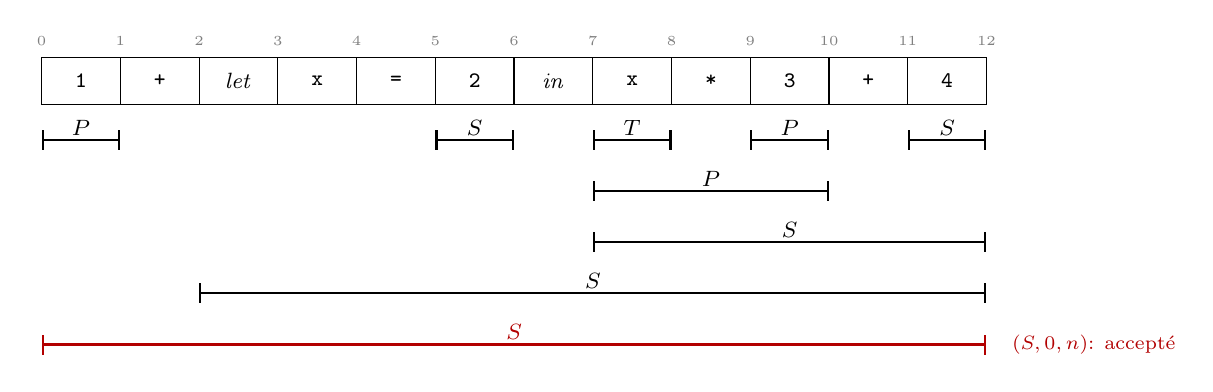
\begin{tikzpicture}[font=\footnotesize, x=1.0cm]
    % token cells
    \foreach \i/\t in {0/{\texttt{1}},1/{\texttt{+}},2/{\textit{let}},3/{\texttt{x}},
                       4/{\texttt{=}},5/{\texttt{2}},6/{\textit{in}},7/{\texttt{x}},
                       8/{\texttt{*}},9/{\texttt{3}},10/{\texttt{+}},11/{\texttt{4}}} {
      \draw (\i,0) rectangle (\i+1,0.6);
      \node at (\i+0.5,0.3) {\t};
    }
    % boundary numbers
    \foreach \i in {0,...,12} {
      \node[anchor=south, font=\tiny, gray] at (\i,0.62) {\i};
    }
    % span bars
    \tikzset{span/.style={|-|, thick}}
    \foreach \a/\b/\lab/\y in {%
      0/1/{$P$}/-0.45, 5/6/{$S$}/-0.45, 7/8/{$T$}/-0.45,
      9/10/{$P$}/-0.45, 11/12/{$S$}/-0.45} {
      \draw[span] (\a,\y) -- (\b,\y);
      \node[anchor=south, inner sep=1.5pt] at ({(\a+\b)/2},\y) {\lab};
    }
    \draw[span] (7,-1.1) -- (10,-1.1);
    \node[anchor=south, inner sep=1.5pt] at (8.5,-1.1) {$P$};
    \draw[span] (7,-1.75) -- (12,-1.75);
    \node[anchor=south, inner sep=1.5pt] at (9.5,-1.75) {$S$};
    \draw[span] (2,-2.4) -- (12,-2.4);
    \node[anchor=south, inner sep=1.5pt] at (7,-2.4) {$S$};
    \draw[span, red!70!black] (0,-3.05) -- (12,-3.05);
    \node[anchor=south, inner sep=1.5pt, red!70!black] at (6,-3.05) {$S$};
    \node[anchor=west, font=\scriptsize, red!70!black] at (12.2,-3.05)
      {$(S,0,n)$: accepté};
  \end{tikzpicture}
\end{figure}

\begin{remark}[Checking the trace]
  Two checks apply to any trace. First, a span always has $i \leq j$: the
  lexème \verb|3| sits at index $9$, so step 2 yields $(9,10,T)$ alongside
  $(9,10,P)$. Second, every justification names productions of the grammar:
  the last step is $S \to P + S$ applied to $(0,1,P)$, $(1,2,+)$ and
  $(2,12,S)$.
\end{remark}

\begin{remark}[Why is this grammar not ambiguous?]
  The answer is that the three non-terminaux are \emph{stratified} exactly as
  in the precedence construction above: $T$ derives a single lexème, $P$
  derives a $*$-chain of $T$s, and $S$ derives a $+$-chain of $P$s or a
  \verb|let|-expression. So for any given span at most one production can apply:
  a span containing a top-level $+$ is not a $P$, and no $P$ or $T$ can start
  with \verb|let|. Where a rule mentions the same non-terminal twice --- $T*P$,
  $P+S$ --- the recursion is on the right only, so the cut is forced at the
  \emph{first} operator of the chain and there is nothing left to choose. Both
  operators therefore come out right-associative.
\end{remark}

\subsection{Utilisation en pratique}
La reconnaissance de mots par CFG est en $O(n^{3} \times |G|)$, cela peut
sembler raisonnable mais :

\begin{itemize}
  \item les fichiers de code contiennent parfois plusieurs milliers de lignes
    (et plus si on compte les entêtes inclus) ;
  \item cela peut faire de l'ordre de la centaine de milliers voire du million
    de symboles ;
  \item un processeur des années 70 faisait $\sim 10^{6}$ opérations par
    seconde $\Rightarrow$ il aurait fallu $30\,000$ ans pour faire $10^{18}$
    opérations ;
  \item un processeur moderne fait $\sim 10^{9}$ opérations par seconde
    $\Rightarrow$ il faut $32$ ans pour faire $10^{18}$ opérations.
\end{itemize}

\begin{remark}
  $10^{18}$ is $n^{3}$ for $n = 10^{6}$, so the two lines are the same
  computation on the same file. The point is the exponent, not the constant:
  four decades of hardware progress moved a cubic algorithm from
  ``geologically impossible'' to ``merely impossible''. Hence les langages
  utilisent souvent des grammaires avec \textbf{test linéaire}
  (\textit{linear test}).
\end{remark}

\begin{figure}[h!]
  \centering
  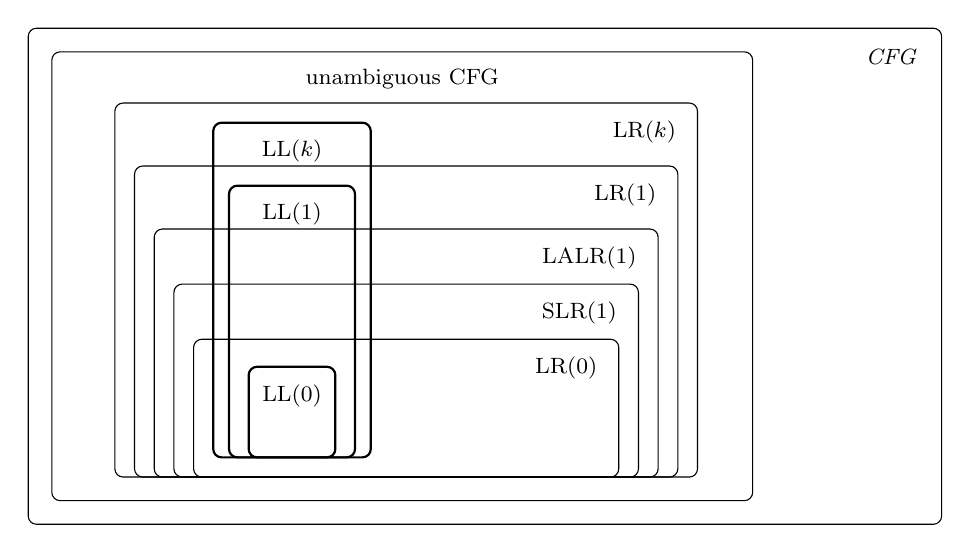
\begin{tikzpicture}[font=\footnotesize]
    \tikzset{cls/.style={draw, rounded corners=3pt}}
    % outermost : CFG
    \draw[cls] (0,0) rectangle (11.6,6.3);
    \node[anchor=north east, font=\footnotesize\itshape] at (11.4,6.15) {CFG};
    % unambiguous CFG
    \draw[cls] (0.3,0.3) rectangle (9.2,6.0);
    \node[anchor=north] at (4.75,5.9) {unambiguous CFG};
    % LR chain
    \draw[cls] (1.1,0.6) rectangle (8.5,5.35);
    \node[anchor=north east] at (8.35,5.25) {LR($k$)};
    \draw[cls] (1.35,0.6) rectangle (8.25,4.55);
    \node[anchor=north east] at (8.1,4.45) {LR($1$)};
    \draw[cls] (1.6,0.6) rectangle (8.0,3.75);
    \node[anchor=north east] at (7.85,3.65) {LALR($1$)};
    \draw[cls] (1.85,0.6) rectangle (7.75,3.05);
    \node[anchor=north east] at (7.6,2.95) {SLR($1$)};
    \draw[cls] (2.1,0.6) rectangle (7.5,2.35);
    \node[anchor=north east] at (7.35,2.25) {LR($0$)};
    % LL chain, crossing the LR boxes on the left
    \draw[cls, thick] (2.35,0.85) rectangle (4.35,5.1);
    \node[anchor=north] at (3.35,5.0) {LL($k$)};
    \draw[cls, thick] (2.55,0.85) rectangle (4.15,4.3);
    \node[anchor=north] at (3.35,4.2) {LL($1$)};
    \draw[cls, thick] (2.8,0.85) rectangle (3.9,2.0);
    \node[anchor=north] at (3.35,1.9) {LL($0$)};
  \end{tikzpicture}
\end{figure}

\noindent Read the picture as inclusions of \emph{grammar} classes, not of
languages: $\text{LR}(0) \subset \text{SLR}(1) \subset \text{LALR}(1) \subset
\text{LR}(1) \subset \text{LR}(k)$, all of them non-ambiguës, and the LL boxes
cut across them --- $\text{LL}(0) \subset \text{LL}(1) \subset \text{LL}(k)$
with each $\text{LL}(i)$ inside the corresponding $\text{LR}(i)$. The
\textit{lookahead} $k$ is the number of lexèmes the parser is allowed to peek at,
and the classes with $k = 1$ are the ones for which parser generators exist.

\subsection{Analyse syntaxique descendante}

Comment reconnaître \emph{rapidement} une telle grammaire ? Take the stratified
expression grammar, reduced to two operators:
\[
  \begin{aligned}
    S_{0} &\to S_{1} + S_{0} & \qquad S_{1} &\to S_{2} * S_{1} & \qquad S_{2} &\to \texttt{int} \\
    S_{0} &\to S_{1}         & \qquad S_{1} &\to S_{2}         &              &
  \end{aligned}
\]

\begin{example}[Recursive descent by hand]
  With two primitives on the lexème stream --- \verb|peek()| donne le prochain
  symbole à lire sans le consommer, \verb|eat()| donne et consomme le prochain
  symbole --- one function per non-terminal suffices.

\begin{lstlisting}[language=Python]
peek() # donne le prochain symbole a lire sans le consommer
eat()  # donne et consomme le prochain symbole

def s0():                def s1():                def s2():
  a = s1()                 a = s2()                 a = peek()
  if peek() != '+':        if peek() != '*':        assert(a == 'int')
    return a                 return a               eat()
  eat()                    eat()                    return a
  return (a,'+',s0())      return (a,'*',s1())
\end{lstlisting}

  Each function returns the subtree it has just recognised; the tuple
  \verb|(a,'+',s0())| \emph{is} the node of the arbre de dérivation. Note that
  the recursive call sits in the returned tuple, i.e.\ at the right of the node,
  matching the right recursion of $S_{0} \to S_{1} + S_{0}$.
\end{example}

\begin{remark}
  This is why the method is called \textbf{descendante} (\textit{top-down}): the
  parser starts at $S$ and descends, choosing a production before it has seen
  what it derives. The CYK algorithm of the previous section is the opposite ---
  bottom-up, combining items already recognised. Analyse syntaxique descendante
  is linear and fits in twelve lines; the price is that the choice of production
  has to be decidable from the next lexème alone, which is exactly the LL(1)
  condition.
\end{remark}

\subsubsection{Pourquoi cela marche et peut-on généraliser ?}
Commençons par réécrire la grammaire, so that the choice is never between two
productions that begin the same way --- \textbf{factorisation à gauche}
(\textit{left factoring}):
\[
  \begin{aligned}
    S_{0} &\to S_{1}F_{0} & \qquad S_{1} &\to S_{2}F_{1} & \qquad S_{2} &\to \texttt{int} \\
    F_{0} &\to +S_{0}     & \qquad F_{1} &\to *S_{1}     &              & \\
    F_{0} &\to \epsilon   & \qquad F_{1} &\to \epsilon   &              &
  \end{aligned}
\]
The common prefix $S_{1}$ of the two $S_{0}$-rules has been pulled out, and what
was the choice between $S_{1} + S_{0}$ and $S_{1}$ has become the choice, inside
$F_{0}$, between consuming a $+$ and producing nothing. The rewritten grammar is
a transcription of the code: the \verb|if peek() != '+': return a| is exactly
$F_{0} \to \epsilon$.

\begin{definition}[Les trois ensembles]
  \leavevmode
  \begin{itemize}
    \item \textit{Null}: the set of non-terminaux $X$ such that
      $X \Rightarrow \epsilon$;
    \item $\mathit{Suivant}(X)$ (\textit{follow}) : les terminaux qui peuvent
      suivre $X$ ;
    \item $\mathit{Premier}(X)$ (\textit{first}) : les terminaux qui peuvent
      commencer un mot dérivé de $X$.
  \end{itemize}
\end{definition}

\begin{remark}
  \textit{Null} is a set of \emph{non-terminaux}. A terminal derives only
  itself, so no \emph{terminal} $X$ satisfies $X \Rightarrow \epsilon$, and a
  \textit{Null} made of terminaux would always be empty. The computed value
  $\{F_{0},F_{1}\}$ below is indeed a set of non-terminaux.
\end{remark}

\begin{example}[The three sets on the factored grammar]
  \[
    \mathit{Null} = \{F_{0}, F_{1}\}
  \]
  \[
    \begin{aligned}
      \mathit{Premier}(S_{i}) &= \{\texttt{int}\} & \qquad
      \mathit{Suivant}(S_{0}) = \mathit{Suivant}(F_{0}) &= \{\} \\
      \mathit{Premier}(F_{0}) &= \{+\}            & \qquad
      \mathit{Suivant}(S_{1}) = \mathit{Suivant}(F_{1}) &= \{+\} \\
      \mathit{Premier}(F_{1}) &= \{*\}            & \qquad
      \mathit{Suivant}(S_{2}) &= \{*, +\}
    \end{aligned}
  \]
  Every $S_{i}$ begins with \verb|int| because every chain bottoms out at
  $S_{2} \to \texttt{int}$. $\mathit{Suivant}(S_{0})$ is empty because $S_{0}$
  is the symbole de départ and nothing follows the whole input.
  $\mathit{Suivant}(S_{2}) = \{*,+\}$ collects $\mathit{Premier}(F_{1}) = \{*\}$
  from $S_{1} \to S_{2}F_{1}$ and, because $F_{1}$ is nullable,
  $\mathit{Suivant}(S_{1}) = \{+\}$ as well.
\end{example}

\begin{definition}[Grammaire LL(1)]
  \textbf{Grammaire LL(1)} : grammaire qui ne contient pas $X \to \alpha$ et
  $X \to \beta$ ($\alpha \neq \beta$) telles que (any one of the following is
  enough) :
  \begin{itemize}
    \item $\alpha$ et $\beta$ dérivent toutes deux $\epsilon$ ;
    \item $\mathit{Premier}(\alpha) \intersect \mathit{Premier}(\beta) \neq \emptyset$ ;
    \item $\alpha$ dérive $\epsilon$ et
      $\mathit{Premier}(\beta) \intersect \mathit{Suivant}(X) \neq \emptyset$.
  \end{itemize}
\end{definition}

\noindent $\Rightarrow$ définition alternative de LL(1) : \textbf{le prochain
symbole détermine la production à utiliser}. Each of the three clauses is one
way for two productions of the same $X$ to be indistinguishable on one lexème
of lookahead --- both empty,
both able to start with the same terminal, or one empty and the other able to
start with something that could equally well have been the continuation after
$X$.\\

The factored grammar above violates none of the three, so it is
\textbf{LL(1)} --- and that is the theorem behind the twelve lines of code: for
an LL(1) grammar the recursive-descent parser is well defined, deterministic,
and runs in time linear in the number of lexèmes.

\subsubsection{Exercice --- un analyseur syntaxique descendant pour la grammaire \texttt{let}}
\begin{problem}
  Comprendre pourquoi cette grammaire n'est pas LL(1) puis la modifier pour la
  rendre LL(1) et enfin écrire un analyseur syntaxique descendant.
  \[
    \begin{aligned}
      S &\to \texttt{let var} = S\ \texttt{in}\ S & \qquad P &\to T   & \qquad T &\to \texttt{var} \\
      S &\to P                                    & \qquad P &\to T*P & \qquad T &\to \texttt{int} \\
      S &\to P+S                                  &          &       &          &
    \end{aligned}
  \]
  Terminaux : \verb|var|, \verb|int|, \verb|+|, \verb|*|, \verb|let|, \verb|=|,
  \verb|in|.
\end{problem}

\begin{example}[Worked answer]
  What follows applies the method of the previous subsection.

  \medskip
  \textbf{Why it fails.} $\mathit{Premier}(P) = \mathit{Premier}(T) =
  \{\texttt{var}, \texttt{int}\}$, so the two productions $S \to P$ and
  $S \to P+S$ have intersecting $\mathit{Premier}$ sets and the second clause of
  the definition fires: on seeing \verb|var| the parser cannot tell which to
  choose. The pair $P \to T$ and $P \to T*P$ fails for the same reason. The
  \verb|let| production is fine --- it is the only one beginning with
  \verb|let|.

  \medskip
  \textbf{The fix.} Left-factor both offending pairs, exactly as $S_{0}$ was
  factored into $S_{0} \to S_{1}F_{0}$:
  \[
    \begin{aligned}
      S &\to \texttt{let var} = S\ \texttt{in}\ S & \qquad P &\to T G     & \qquad T &\to \texttt{var} \\
      S &\to P F                                  & \qquad G &\to *P      & \qquad T &\to \texttt{int} \\
      F &\to +S                                   & \qquad G &\to \epsilon &         & \\
      F &\to \epsilon                             &          &            &          &
    \end{aligned}
  \]
  Now $\mathit{Premier}(\texttt{let} \dots) = \{\texttt{let}\}$ is disjoint from
  $\mathit{Premier}(PF) = \{\texttt{var},\texttt{int}\}$; $F$ and $G$ each offer
  a production starting with a distinct operator against an
  $\epsilon$-production, and $+ \notin \mathit{Suivant}(F)$,
  $* \notin \mathit{Suivant}(G)$, so the third clause does not fire either.

  \medskip
  \textbf{The parser.}
\begin{lstlisting}[language=Python]
def s():
  if peek() == 'let':
    eat()                       # let
    v = eat()                   # var
    eat()                       # =
    e1 = s()
    eat()                       # in
    return ('let', v, e1, s())
  a = p()
  if peek() != '+':             # F -> epsilon
    return a
  eat()
  return (a,'+',s())            # F -> + S

def p():
  a = t()
  if peek() != '*':             # G -> epsilon
    return a
  eat()
  return (a,'*',p())            # G -> * P

def t():
  a = peek()
  assert(a == 'var' or a == 'int')
  eat()
  return a
\end{lstlisting}
  One function per non-terminal of the \emph{unfactored} grammar; the factored
  $F$ and $G$ appear as the trailing \verb|if| inside \verb|s()| and \verb|p()|
  rather than as functions of their own, which is the usual way the
  factorisation is written back into code.
\end{example}

\subsection{De nombreuses classes\dots}
Il existe d'autres classes intéressantes, considérons maintenant les CFG où
toutes les productions sont de la forme
\[
  N \to \Sigma \times N \union \epsilon ,
\]
that is, every right-hand side is either a terminal followed by a single
non-terminal, or empty.

\begin{theorem}
  These are exactly the \textbf{langages réguliers} (\textit{regular
  languages}).
\end{theorem}

\begin{remark}
  Such grammars are the \textbf{right-linear} ones, and the correspondence with
  automates finis is immediate: read each non-terminal as an état, each rule
  $N \to cM$ as a transition $N \xrightarrow{\,c\,} M$, and each rule
  $N \to \epsilon$ as ``$N$ is accepting''. The symbole de départ is the état
  initial. Nothing is lost and nothing is added, which is why the next chapter
  can speak of automates and of grammars interchangeably.
\end{remark}

\begin{figure}[h!]
  \centering
  \begin{tikzpicture}[font=\small, node distance=2.4cm,
                      every state/.style={minimum size=7mm, inner sep=1pt}]
    \node[state, initial, initial text={}] (N) {$N$};
    \node[state, accepting, right=of N] (M) {$M$};
    \path[->] (N) edge node[above] {$c$} (M);
  \end{tikzpicture}
\end{figure}

\noindent The rules $N \to cM$ and $M \to \epsilon$, read as an automate.

\begin{conclusion}
  Four thresholds structure the chapter, and each one is a restriction paid for
  with an algorithm. General grammaires formelles: problème de l'appartenance
  indécidable. Restrict the left-hand side to a single non-terminal and one gets
  the grammaires non contextuelles, where the problème de l'appartenance is
  decided in $O(n^{3} \times |G|)$ by saturating the relation $\mathit{match}$
  --- CYK --- after binarising the productions. Cubic is still hopeless on a
  file of a million lexèmes, so restrict further to the grammars whose next
  production is determined by the next lexème: LL(1), tested with
  \textit{Null}, $\mathit{Premier}$ and $\mathit{Suivant}$, parsed in linear
  time by one recursive function per non-terminal. Restrict once more, to
  right-linear productions, and one has fallen out of analyse syntaxique
  altogether into the langages réguliers and automates finis --- which is where
  the lexeur lives, and where the next chapter begins.\\

  The recurring technique, across all four levels, is \emph{rewriting the
  grammar rather than the parser}: stratify by precedence to fix associativité,
  introduce a closed non-terminal to fix the dangling \verb|else|, binarise to
  fit CYK, left-factor to fit LL(1). The language recognised never changes; only
  the shape of the trees, and the algorithm that can afford to build them.
\end{conclusion}
